\documentclass[%
 reprint,
%superscriptaddress,
%groupedaddress,
%unsortedaddress,
%runinaddress,
%frontmatterverbose, 
%preprint,
%showpacs,preprintnumbers,
%nofootinbib,
%nobibnotes,
%bibnotes,
 amsmath,amssymb,
 aps,
%pra,
%prb,
%rmp,
%prstab,
%prstper,
%floatfix,
]{revtex4-1}

\usepackage{graphicx}% Include figure files
\usepackage{dcolumn}% Align table columns on decimal point
\usepackage{bm}% bold math
\usepackage{hyperref}% add hypertext capabilities
%\usepackage[mathlines]{lineno}% Enable numbering of text and display math
%\linenumbers\relax % Commence numbering lines

%\usepackage[showframe,%Uncomment any one of the following lines to test 
%%scale=0.7, marginratio={1:1, 2:3}, ignoreall,% default settings
%%text={7in,10in},centering,
%%margin=1.5in,
%%total={6.5in,8.75in}, top=1.2in, left=0.9in, includefoot,
%%height=10in,a5paper,hmargin={3cm,0.8in},
%]{geometry}

\begin{document}

%\preprint{APS/123-QED}

\title{Nuclear astrophysical implications of a reduction in the fine structure constant}% 
\thanks{Midterm paper for PHYS-554: Nuclear Astrophysics}%

\author{Adam Richie-Halford}
\email{richford@uw.edu}
\affiliation{
 Department of Physics \\
 University of Washington \\
 Seattle, Washington 98195, USA
}

\date{\today}% It is always \today, today,
             %  but any date may be explicitly specified

\begin{abstract}
I discuss the implications of a reduction in the fine structure constant in a newly discovered parallel universe. This reduction in $\alpha$ is equivalent to a reduction in the proton charge, a reduction in the Coulomb barrier for some nuclear reactions, and an increase in the neutron-proton mass difference. I discuss the implications for nuclear masses, nuclide stability, big bang nucleosynthesis, the stellar p+p reaction rates, and solar neutrino emission.
%\begin{description}
%\item[Usage]
%Secondary publications and information retrieval purposes.
%\item[Structure]
%You may use the \texttt{description} environment to structure your abstract;
%use the optional argument of the \verb+\item+ command to give the category of each item. 
%\end{description}
\end{abstract}

\pacs{Valid PACS appear here}% PACS, the Physics and Astronomy
                             % Classification Scheme.
%\keywords{Suggested keywords}%Use showkeys class option if keyword
                              %display desired
\maketitle

%\tableofcontents

\section{\label{sec:intro}Introduction}

The recent discovery of a parallel universe\cite{ReddyMidterm} has spurred speculation about its nuclear astrophysical properties. Remarkably, this parallel universe has identical fundamental constants $\hbar$ and $c$ as well as identical parameters of QCD and of the weak interactions. The quark and lepton masses are also identical. The only difference in fundamental constants is that of the fine structure constant, which in the parallel universe is given by
\begin{equation}
	\widetilde{\alpha} = \alpha / 2 = 1 / 274.
\end{equation}
This reduction in $\alpha$ also alters the neutron-proton mass difference, which is given by\cite{ReddyMidterm}
\begin{equation}
	\Delta \widetilde{m} = \widetilde{m_n} - \widetilde{m_p} \approx 2 \; \text{MeV}.
\end{equation}

In this paper, I discuss the implications of this reduction in $\alpha$. In Section \ref{sec:masses}, I discuss the effect on nuclear masses and calculate the $A$ and $Z$ numbers of the most stable nucleus using the semi-empirical mass formula. In Section \ref{sec:bbn}, I discuss the implications for big bang nucleosynthesis (BBN) and in particular for the relative abundance of ${}^4\text{He}$ during BBN. Lastly, in Section \ref{sec:neutrinos}, I discuss the effect of changing $\alpha$ on stellar nuclear processes and on solar neutrino emission.

Throughout this paper, I use tilde variable (e.g. $\widetilde{x}$ rather than $x$) to refer to quantities calculated for the parallel universe. In section \ref{sec:neutrinos}, I use the dimensionless constant $\xi \equiv \widetilde{\alpha} / \alpha$ to relate physical quantities in the parallel universe to those in our own. In the interest of furthering open science, I have included a link to an executable jupyter notebook\cite{jupyter_notebook} which recapitulates the calculations in this paper.

\section{\label{sec:results}Results}

\subsection{\label{sec:masses}Effects on nuclear masses}

\subsubsection{\label{sec:table_of_nuclides}Nuclide stability}

Ignoring shell effects and pairing effects, one may approximate the binding energy of a nucleus using the Weizs\"acker mass formula\cite{1935ZPhy...96..431W}
\begin{equation}
	B(A, Z) = a_V A - a_S A^{2/3} - a_C \frac{Z (Z-1)}{A^{1/3}}
	- a_{\text{sym}} \frac{(N-Z)^2}{A}.
	\label{eq:weizsacker}
\end{equation}

The volume and surface terms are based on the strong nuclear force, so they should remain unchanged in the parallel universe. Using one popular set of values for the Weizs\"acker coefficients\cite{wong1990introductory}, we may take
\begin{equation}
	a_V = 15.5 \; \text{MeV} \\
	a_S = 16.8 \; \text{MeV}.
\end{equation}
Similarly, the symmetry term is not based on the fundamental forces but rather on the Pauli exclusion principle. So we may use the value of $a_{\text{sym}} = 23 \; \text{MeV}$ to be the same as in our universe.\cite{wong1990introductory}

In our universe, $a_C = 0.72 \; \text{MeV}$. We can approximate $a_C$ by equating it with the energy of a charged sphere,
\begin{equation}
	\frac{3}{5} \frac{Z^2 e^2}{4 \pi \epsilon_0 R} = 
	\frac{3}{5} \frac{Z^2 \alpha \hbar c}{R}
	\approx a_C \frac{Z(Z-1)}{A^{1/3}}.
\end{equation}

So if the value of the fine structure constant were reduced by one-half, then the Coulomb term in the mass formula would also be reduced by the same amount,
\begin{equation}
	\alpha \rightarrow \widetilde{\alpha} = \frac{\alpha}{2}
	\quad \Longrightarrow \quad
	a_C \rightarrow \widetilde{a}_C = \frac{a_C}{2}.
\end{equation}
Thus, in the parallel universe, we have $\widetilde{a}_C = 0.36 \; \text{MeV}$.

To gain intuition about the differences between our universes, I plot the nuclide valley of stability by plotting a contour of the neutron and proton drip lines using the mass formula in Eq\eqref{eq:weizsacker}. The drip lines will be determined by the point at which the separation energies $S_p$ and $S_n$ vanish,
\begin{align}
	S_n &= E_B(N+1, Z) - E_B(N, Z) = 0, \\
	S_p &= E_B(N, Z+1) - E_B(N, Z) = 0.
\end{align}
In the region of stability, $S_n S_p > 0$, so we may plot contour lines of the quantity $S_n S_p$ and restrict to positive values to visualize the table of nuclides. In Figure \ref{fig:nuclides}, I use this technique to plot the stable nuclides for $0 < N < 100$ and $0 < Z < 100$, both for our universe and for ``their" universe.

\begin{figure}[h!]
	\centering
	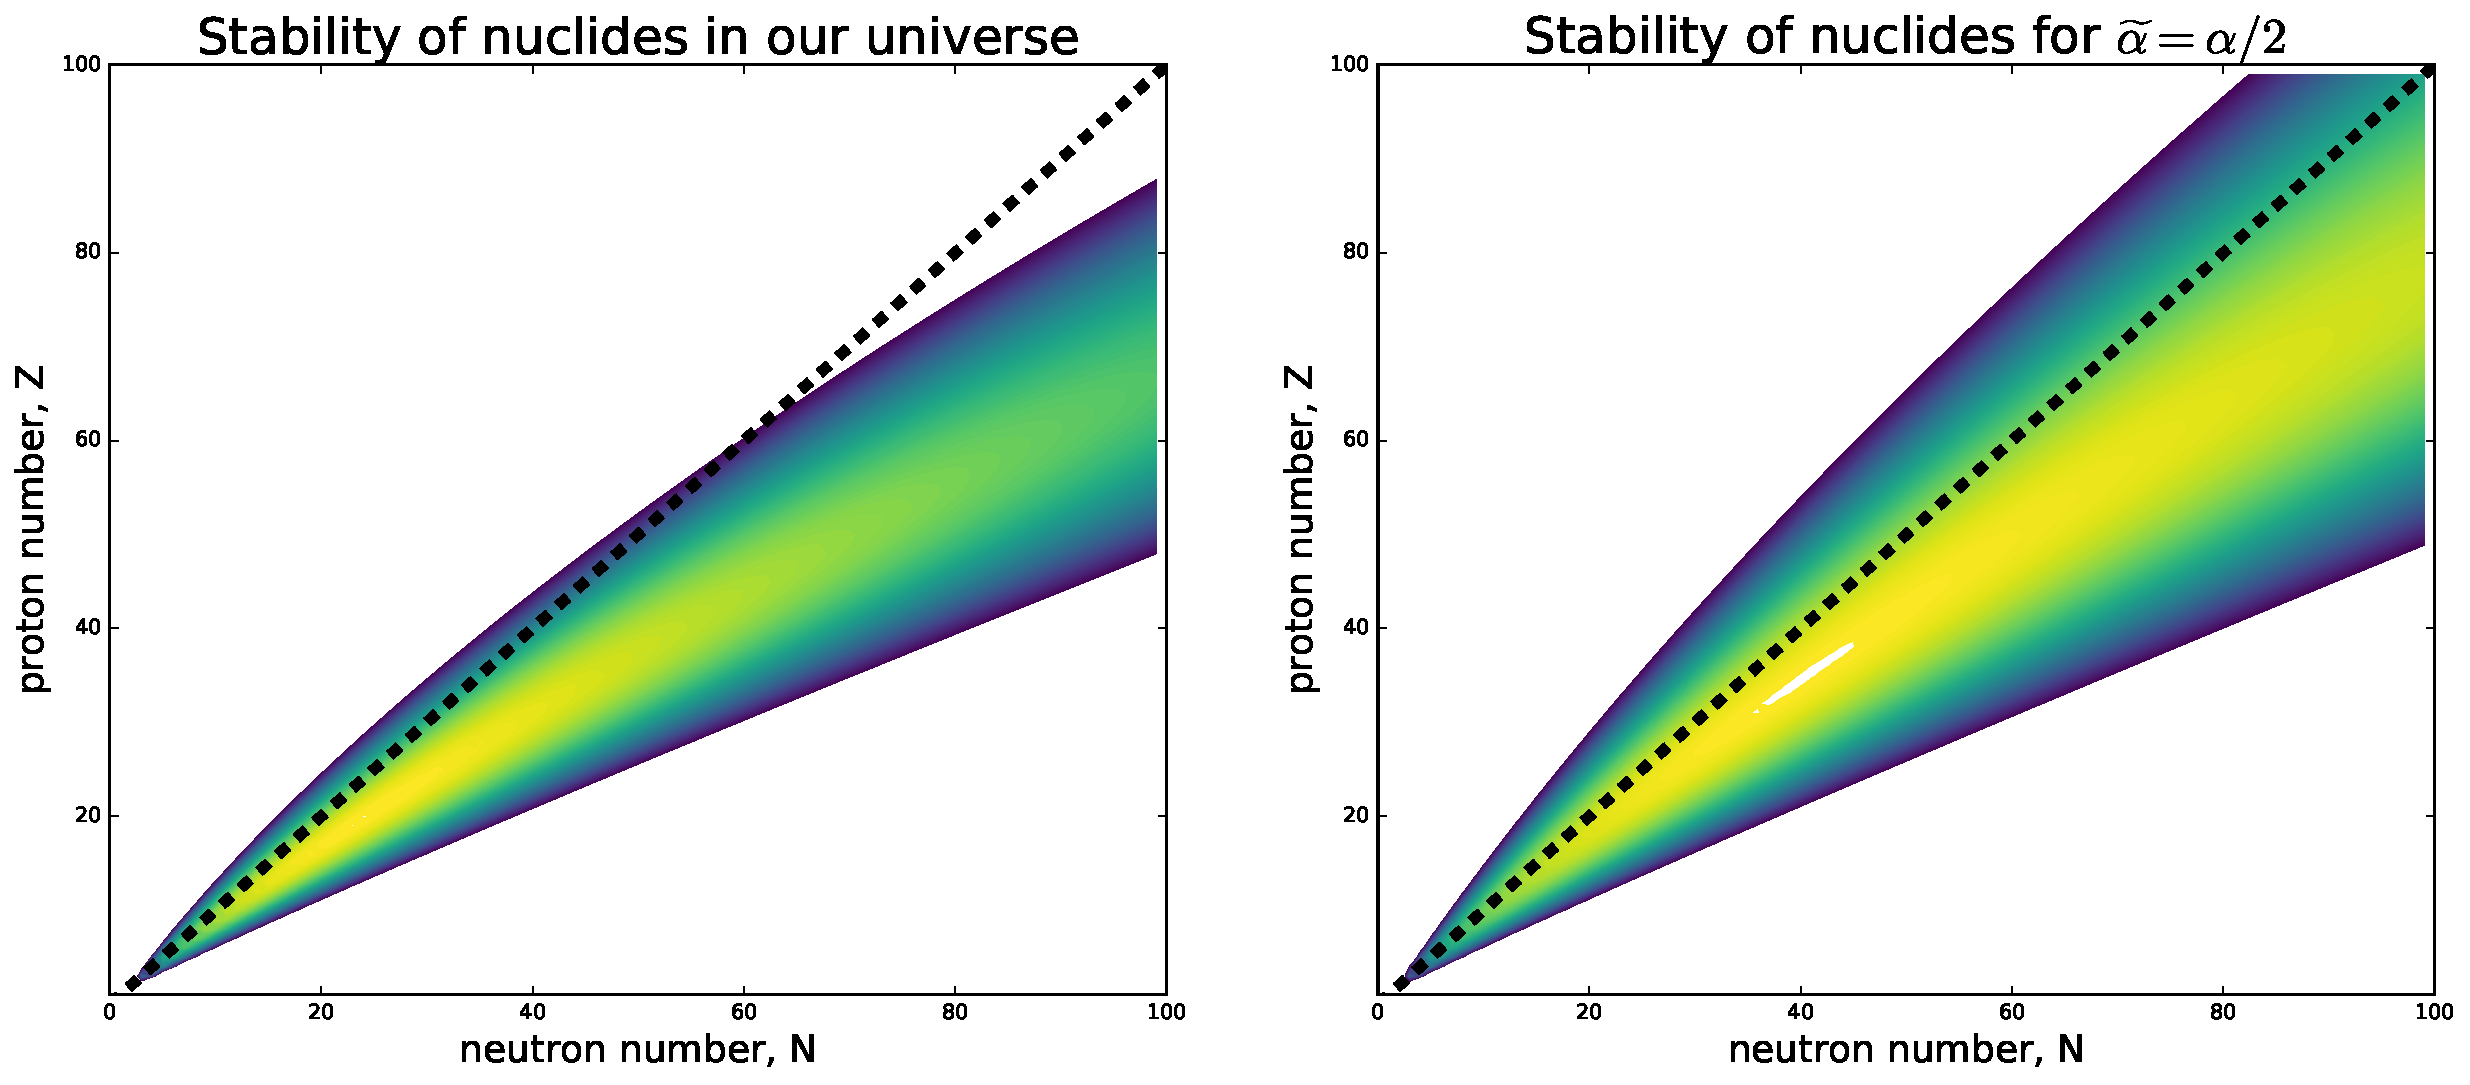
\includegraphics[width=\linewidth]{fig/nuclides.pdf}
	\caption{\label{fig:nuclides}Table of nuclides in our universe (left) and ``their" universe (right). I plot a contour of $S_n S_p$ to visualize the valley of stability in both universes. The dotted black line shows the $A=Z$ reference line. In our universe, larger nuclei have higher proton-neutron asymmetry in order to compensate for Coulomb repulsion. As expected, in the parallel universe, nuclides have similar numbers of protons and neutrons due to the reduced proton charge.}
\end{figure}

The parallel universe's valley of stability follows the $A=Z$ reference line much more closely than in our universe. This is as expected, since the reduction in $\alpha$ reduces the proton charge, and therefore the Coulomb repulsion inside each nucleus.

\subsubsection{\label{sec:stable_nuclei}Identifying stable nuclei}

For a fixed nucleon number, A, one can find the optimal proton number by maximizing the binding energy
\begin{equation}
	\left. \frac{d E_b}{d Z}\right|_{\text{fixed A}} =
	- a_C \frac{2Z - 1}{A^{1/3}}
	+ a_{\text{sym}} \frac{4 (A - 2Z)}{A}
	\overset{!}{=} 0.
	\label{eq:constraint}
\end{equation}

Solving Eq\eqref{eq:constraint} for $Z$ yields
\begin{equation}
	Z_\text{optimal} = \frac{2 a_\text{sym} A^{4/3} + a_C A / 2}{
	4 a_\text{sym} A^{1/3} + a_C A}
	= A - N_\text{optimal},
\end{equation}
and inserting this into Eq\eqref{eq:weizsacker} yields an equation for the binding energy as a function of $A$ only. I then solve this equation numerically to find $A_\text{max}$, the nucleon number that maximizes the binding energy per nucleon $E_b(A) / A$.\cite{jupyter_notebook}. This yields the $A$ value of the most stable nucleus.

In our universe, using the Weizs\"acker formula, the most stable nucleus has $(A, Z) = (57, 26)$ with a binding energy per nucleon of 8.82 MeV. In ``their" universe, the most stable nucleus has $(A, Z) = (98, 45)$ with a binding energy per nucleon of 10.13 MeV. In Figure \ref{fig:binding_energy}, I plot the binding energy per nucleon as a function of $A = N_\text{optimal} + Z_\text{optimal}$. Because of the reduction in Coulomb repulsion in the parallel universe, $A_\text{max}^{(\widetilde{\alpha})} > A_\text{max}^{(\alpha)}$.

\begin{figure}[h!]
	\centering
	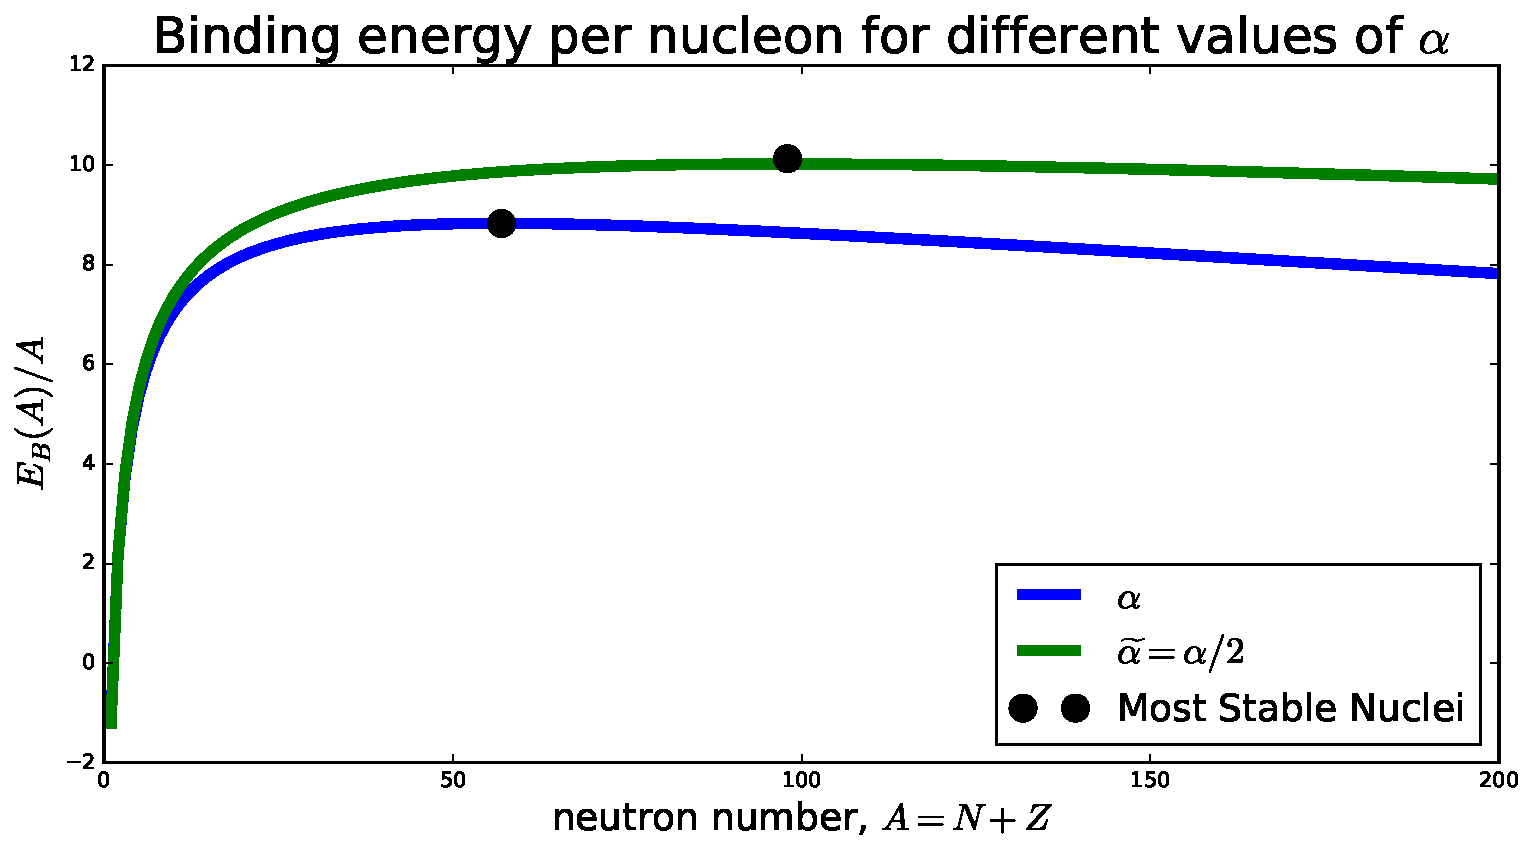
\includegraphics[width=\linewidth]{fig/binding_energy.pdf}
	\caption{\label{fig:binding_energy}Binding energy per nucleon as a function of nucleon number, $A = N_\text{optimal} + Z_\text{optimal}$.}
\end{figure}

\subsubsection{\label{sec:stable_isotopes}Stable isotopes}

Having identified the most stable nucleus, let us turn our attention to the most stable isotopes in our universe and in ``theirs." I numerically find the neutron number $N$ that maximizes the binding energy per nucleon for each $Z$ value\cite{jupyter_notebook} and plot the results in Figure \ref{fig:stable_isotopes}. In our universe, as one increases the proton number, more and more neutrons are needed so that the attractive short-range strong force overcomes the Coulomb repulsion of the protons. In ``their" universe, the smaller proton charge means that fewer neutrons are required for stability

\begin{figure}[h!]
	\centering
	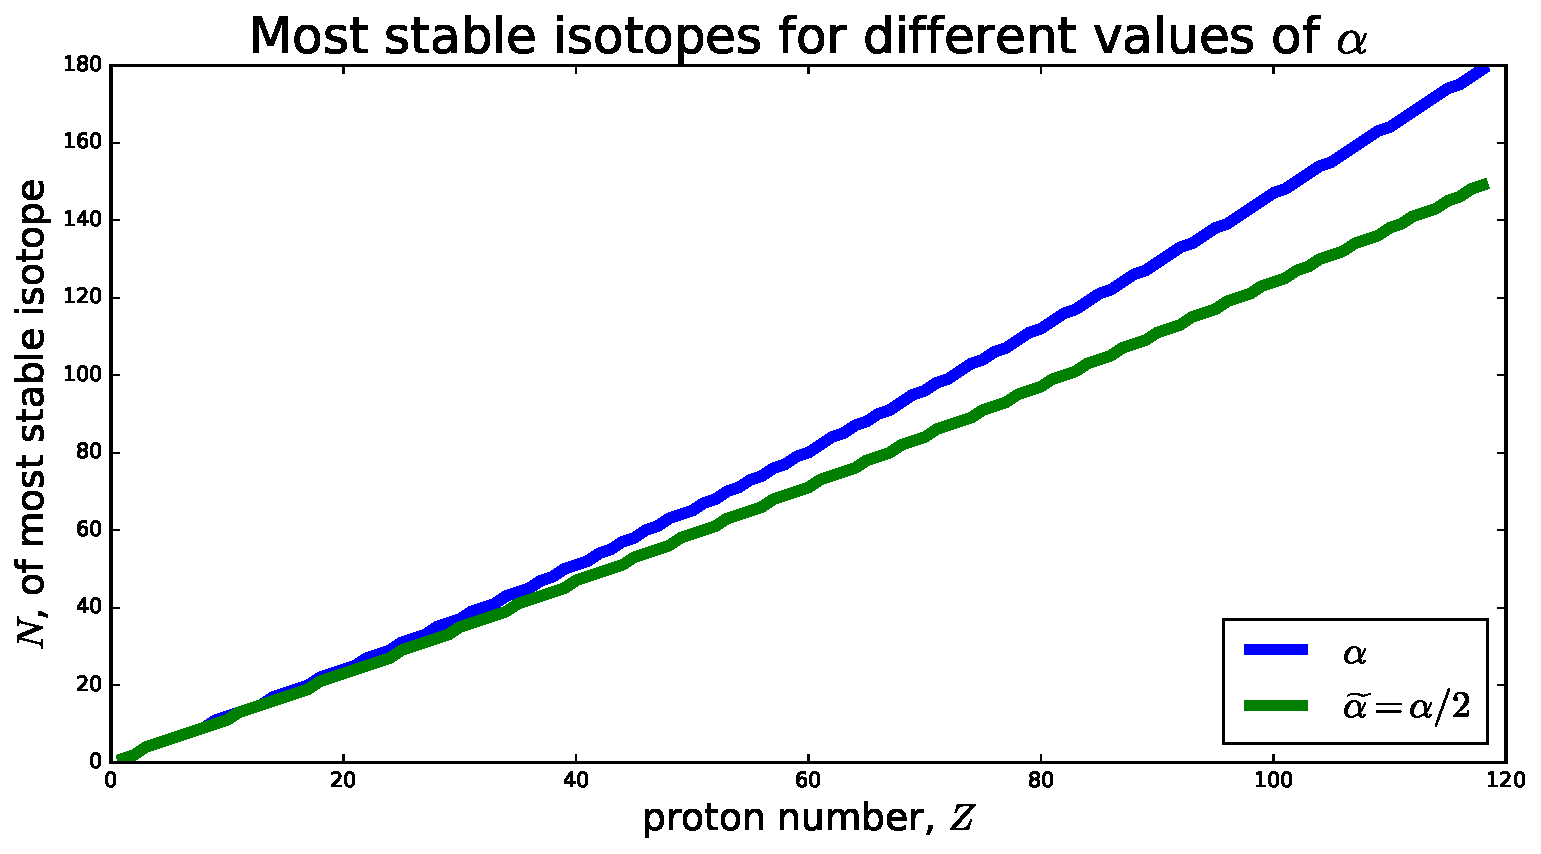
\includegraphics[width=\linewidth]{fig/stable_isotopes.pdf}
	\caption{\label{fig:stable_isotopes}The neutron number, $N$, of the most stable isotopes in our universe and in ``theirs." In our universe, more neutrons are needed so that the attractive short-range strong force overcomes the Coulomb repulsion of the protons. In ``their" universe, the smaller proton charge means that fewer neutrons are required for stability.}
\end{figure}

\subsection{\label{sec:bbn}Effects on big bang nucleosynthesis (BBN)}

In the early universe, for a given $\mu$ and $T$, the nucleon densities are given by\cite{ReddyLectureNotes}
\begin{align}
	n_n = 2 \left( \frac{m_n T}{2 \pi} \right)^{3/2}
	\exp\left( \frac{-m_n}{T} \right) \exp\left( \frac{\mu_n}{T} \right), \\
	n_p = 2 \left( \frac{m_p T}{2 \pi} \right)^{3/2}
	\exp\left( \frac{-m_p}{T} \right) \exp\left( \frac{\mu_p}{T} \right).
\end{align}

For $T \ge 0.7 \; \text{MeV}$, the weak reaction rates that exchange protons and neutrons are fast compared to the expansion rate of the universe, so the difference in neutron and proton chemical potentials is negligible compared to their mass difference. So we can approximate the neutron-proton number density ratio as
\begin{equation}
	\frac{n_n}{n_p} \approx \exp \left( \frac{- \Delta m}{T} \right),
\end{equation}
where $\Delta m = m_n - m_p$.\cite{ReddyLectureNotes}

In the early universe, the temperature is very hot and neutrons and protons are roughly equally numerous. As the temperature of the universe cools below $\Delta m$, free neutrons begin to decay at a rate faster than they are produced by weak reactions. So the neutron fraction decreases until "neutron-proton freeze-out," which occurs at a temperature where the rate of weak reactions is equal to the expansion rate of the universe,\cite{CAMPBELL1995429}
\begin{equation}
	\sqrt{G_N N} T_f^2 \sim H(T_f) = \Gamma_\text{weak} (T_f) \sim G_F^2 T_f^5.
\end{equation}

Since the alternate universe has the same expansion rate and weak interaction parameters as our universe, we may take $T_f$ to be the same that is in our universe ($T_f = 0.7\; \text{MeV}$).

After freeze-out, we can approximate the neutron-proton number density ratio as fixed. This ratio remains fixed until light-element synthesis, when deuterium becomes stable and nearly all of the neutrons are synthesized into ${}^4\text{He}$.\cite{PhysRevD.65.123511}

The mass fraction of ${}^4\text{He}$ is then
\begin{align}
	X_\text{He} &= 
	\frac{n_\text{He} m_\text{He}}{n_\text{He} m_\text{He} + n_\text{H} m_\text{H}} \\
	&\approx \frac{4 n_\text{He} m_p}{4 n_\text{He} m_p + n_\text{H} m_p}
	= \frac{4 n_\text{He}}{4 n_\text{He} + n_\text{H}},
\end{align}
where I have used the approximations $m_\text{H} \approx m_p$ and $m_\text{He} \approx 4 m_p$. Assuming that all of the neutrons are sythesized into ${}^4\text{He}$ we can write $n_\text{He} = n_n / 2$, where $n_n$ is the freeze-out number density of neutrons. So we have
\begin{equation}
	X_\text{He} = \frac{2 n_n}{2 n_n + n_\text{H}}.
\end{equation}
Finally, the synthesis of ${}^4\text{He}$ will consume an equal amount of neutrons and protons. So the remaining hydrogen number density will be simply $n_\text{H} = n_p - n_n$, where $n_p$ is the freeze-out number density of protons. This yields
\begin{equation}
	X_\text{He} = \frac{2 n_n}{2 n_n + n_p - n_n}
	= \frac{2 \frac{n_n}{n_p}}{1 + \frac{n_n}{n_p}},
\end{equation}
where again, $n_n$ and $n_p$ are taken at freeze-out. Inserting the freeze-out number density ratio results in
\begin{equation}
	X_\text{He} =
	\frac{2 \exp \left( \frac{- \Delta m}{T_f} \right)}{1 + \exp \left( \frac{- \Delta m}{T_f} \right)}.
\end{equation}

Plugging in the mass differences for our universe and the parallel universe yields
\begin{align}
	X_\text{He}(\Delta m \approx 2 \; \text{MeV}) \approx 0.109 \\
	X_\text{He}(\Delta m \approx 1.29 \; \text{MeV}) \approx 0.273
\end{align}

The change in fine structure constant in the parallel universe reduces the helium abundance during BBN because the increased neutron-proton mass difference causes the neutron fraction to decay more quickly before freeze-out.

\subsection{\label{sec:neutrinos}Effects on the p+p reaction and solar neutrino emission}

Nuclear reactions in stars are governed by a competition between an attractive short-range nuclear potential and the long range Coulomb potential. Consider two nuclei with radii $R_1 \approx 1.4 A_1^{1/3}$ fm and $R_2 \approx 1.4 A_2^{1/3}$ fm at a separation distance of $R = R_1 + R_2$ (i.e. overlap distance). The Coulomb potential at this distance is then
\begin{equation}
    V_C = \frac{Z_1 Z_2 \alpha \hbar c}{
    1.4 \left(A_1^{1/3} + A_2^{2/3} \right) \; \text{fm}}
    \approx
    \xi \frac{Z_1 Z_2}{
    \left(A_1^{1/3} + A_2^{2/3} \right)} \; \text{MeV},
\end{equation}
where $\xi = 1$ in our universe and $\xi = 1/2$ in the parallel universe.

Even when $\xi = 1/2$, $V_C$ will be much larger than the thermal energy of particles in main sequence stars (usually $T \simeq 0.27 - 2.7$ keV). So even in the parallel universe, the nuclei must still tunnel through the Coulomb barrier in order to fuse.

The rate of a reaction $1 + 2 \rightarrow 3 + 4 + \ldots$ in a stellar plasma is given by
\begin{equation}
    r_{12} = \frac{n_1 n_2}{1 + \delta_{12}} \langle \sigma v\rangle,
\end{equation}
where $\langle \sigma v \rangle$ is the thermally averaged cross-section,
\begin{equation}
    \langle \sigma v \rangle = \sqrt{\frac{8}{\mu \pi}}
    \frac{1}{T^{3/2}} \displaystyle \int_0^\infty
    dE \; S(E) \; \exp \left(
        - \frac{E}{T} - \frac{b}{\sqrt{E}}
    \right),
\end{equation}
where $b = 2 \pi \sqrt{2 \mu} Z_1 Z_2 \alpha \hbar c$. The cross-section is exponentially suppressed at high energy by the Boltzmann distribution and also at low energy by the Coulomb barrier. The region of energies where the cross-section is high is called the Gamow window, which peaks at $E = E_0$ and has a width of $\Delta$, with
\begin{equation}
    E_0 = \left( \frac{b T}{2} \right)^{2/3} \\
    \Delta = \frac{4}{\sqrt{3}} \sqrt{E_0 T}.
\end{equation}
If the variation of $S(E)$ is small in the interval $E = E_0 \pm \Delta$, we can write the thermally averaged cross-section as
\begin{equation}
    \langle \sigma v \rangle = \left( \frac{2}{\pi \mu T} \right)^{1/2}
    \left( \frac{\Delta}{T} \right) S(E_0)
    \exp \left( - \frac{3 E_0}{T} \right).
\end{equation}

With a reduced value of $b \propto \alpha$, we expect that the Gamow window will become smaller and move to lower energies.

Next, I parameterize $\widetilde{\alpha} = \xi \alpha$ so that $\xi = 1$ in our universe and $\xi = 1/2$ in the parallel universe. The goal here is to find a relationship between the thermally averaged cross-section in our universe and in ``theirs". Using $\xi$, we can write the thermally averaged cross-section as
\begin{align}
    \langle \widetilde{\sigma v} \rangle
    &= \left( \frac{2}{\pi \mu T} \right)^{1/2}
    \left( \frac{\xi^{1/3} \Delta}{T} \right)
    S\left(\xi^{2/3} E_0 \right)
    \exp \left( -\frac{3 \xi^{2/3} E_0}{T} \right) \\
    &= \xi^{1/3} \frac{S(\xi^{2/3} E_0)}{S(E_0)}
    \exp \left( - \frac{3 (\xi^{2/3} - 1) E_0}{T} \right)
    \langle \sigma v \rangle.
    \label{eq:thermal_average_xc}
\end{align}

Consider the proton-proton reaction
\begin{equation}
    p + p \rightarrow d + e^{+} + \nu_e,
\end{equation}
which is the main source of solar neutrino production. Using Eq\eqref{eq:thermal_average_xc}, the p+p reaction rate for arbitrary values of $\xi$ can be related to the rate of reaction in our universe by
\begin{equation}
    \widetilde{r}_{pp} = \xi^{1/3} \frac{S(\xi^{2/3} E_0)}{S(E_0)}
    \exp \left( - \frac{3 (\xi^{2/3} - 1) E_0}{T} \right)
    r_{pp}.
\end{equation}
At the core of the sun we have $E_0 / T \sim 4.57$ and $E_0 \sim 5.9 \; \text{keV}$.\cite{HaxtonLectureNotes}
So the width of the Gamow window for p+p reactions in the sun is
\begin{equation}
    \Delta = \frac{4}{\sqrt{3}} \frac{E_0}{\sqrt{4.57}}
    \approx 6.37 \; \text{keV}.
\end{equation}
For $\xi = 1/2$, we see that $\xi^{2/3} E_0 \approx 3.72 \; \text{keV}$ is well within the Gamow window $E_0 \pm \Delta$. Then we can assume that the variation in $S(E)$ is small between $E = E_0$ and $E = \xi^{2/3} E_0$. I therefore drop the ratio of S-factors from the rate equation,
\begin{equation}
    \widetilde{r}_{pp} = \xi^{1/3}
    \exp \left( - \frac{3 (\xi^{2/3} - 1) E_0}{T} \right)
    r_{pp}.
\end{equation}
For the core of the sun, with $E_0 / T \sim 4.57$ and $\xi = 1/2$, we have
\begin{equation}
    \widetilde{r}_{pp} = 126.75 \; r_{pp}.
    \label{eq:rpp_ratio}
\end{equation}
In our universe, in the core of the sun, the p+p rate is $r_{pp} \sim 0.5 \times 10^8 / \text{cm}^3 / \text{sec}$.\cite{HaxtonLectureNotes} So the p+p rate in the parallel universe is
\begin{equation}
    \widetilde{r}_{pp} = \frac{6.34 \times 10^9}{\text{cm}^3 \; \text{sec}}.
\end{equation}

In addition to the change in emission rate, the spectrum of solar neutrinos will narrow to accommodate the larger neutron-proton mass difference. The allowed energies for p+p neutrinos are $0 \le E_\nu \le Q$, where
\begin{align}
	Q &= 2 m_p - m_D = 2 m_p - m_n - m_p + B(1, 1) \\
	&= B(1, 1) - \Delta \widetilde{m}.
\end{align}
With $N = 1$ and $Z = 1$ for the deuteron, the Coulomb and asymmetry terms drop out from the Weizs\"acker mass formula in Eq\eqref{eq:weizsacker} so the contribution to $Q$ from the binding energy of the deuteron is the same in both universes. The narrowing of the neutrino spectrum in the parallel universe is due entirely to the increase in $\Delta \widetilde{m}$.

We note here that this analysis depends on how one defines the $Q$ value. If we define
\begin{align}
	Q &= 2 m_p - m_D - m_e = 2 m_p - m_n - m_p + B(1, 1) - m_e \\
	&= B(1, 1) - \Delta \widetilde{m} - m_e,
\end{align}
then we get a negative $Q$ value ($Q \approx - 311 \; \text{keV}$) for the reaction $p + p \rightarrow d + e^+ + \nu_e$. So it appears that the $p+p$ reaction is not allowed, even with the addition of the sun's $\sim 6$ keV thermal energy. Then the dominant neutrino producing reaction will be the pep reaction,
\begin{equation}
	p + e^- + p \rightarrow d + \nu_e.
\end{equation}
In our universe, this reaction accounts for only 0.25\% of solar neutrino production. In the parallel universe it will be the dominant source. In this paper, I assume that the analysis performed for the p+p reaction will still hold (qualitatively) for the pep reaction. That is, the lowered Coulomb barrier will increase the reaction rate. The proof will look slightly different since pep is a three-body reaction. I leave this as an exercise to the reader.

To estimate the effect on the lifetime of the sun, I assume that we are still dealing with the p+p reaction. Then the time scale for burning hydrogen in the parallel universe's sun is\cite{HaxtonLectureNotes}
\begin{equation}
    \widetilde{\tau}_\text{sun} = \frac{\tau_\text{sun}}{126.75}
    = \frac{8.6 \; \text{billion years}}{126.75}
    = 67.85 \; \text{million years}.
    \label{eq:tau_sun_ratio}
\end{equation}
From Eqs\eqref{eq:rpp_ratio}-\eqref{eq:tau_sun_ratio}, we see that the lowering of the Coulomb barrier in the parallel universe leads to an increase in the cross-section and therefore an increase reaction rate for the p+p reaction and the creation of solar $\nu_e$ neutrinos. As a result, the parallel universe's sun burns out faster, with a lifetime of only 67.85 million years. Obviously, the switch to the pep reaction as the main neutrino source obviates this lifetime estimate. The qualitative behavior is however the same.

\section{\label{sec:conclusion}Conclusion}

The reduction of the fine structure constant in the parallel universe has some striking effects. In section \ref{sec:masses}, I used the Weizs\"acker mass formula to show that the reduction in proton charge favors stable nuclei with more symmetric neutron and proton numbers. It brings the valley of stability closer to the $N = Z$ line and makes larger nuclei more stable. In section \ref{sec:bbn}, I discussed implications for BBN and showed that the larger neutron-proton mass difference led to an accelerated decay of the neutron fraction before neutron-proton freeze-out. This in turn led to a lower abundance of ${}^4\text{He}$ than in our universe. Lastly, in section \ref{sec:neutrinos}, I showed that the reduced Coulomb barrier in the parallel universe led to a solar p+p reaction rate that is two orders of magnitude larger than that of our universe. I then argued that the negative $Q$ value of this reaction means that p+p will no longer be the main source of solar neutrinos. Instead the pep reaction will dominate neutrino production. However, I argued that the increase in the reaction rate would still hold for the pep reaction.

\bibliographystyle{apsrev4-1}
\bibliography{midterm} 

\end{document}